% Included by chapters/comparison_existing_approaches.tex.
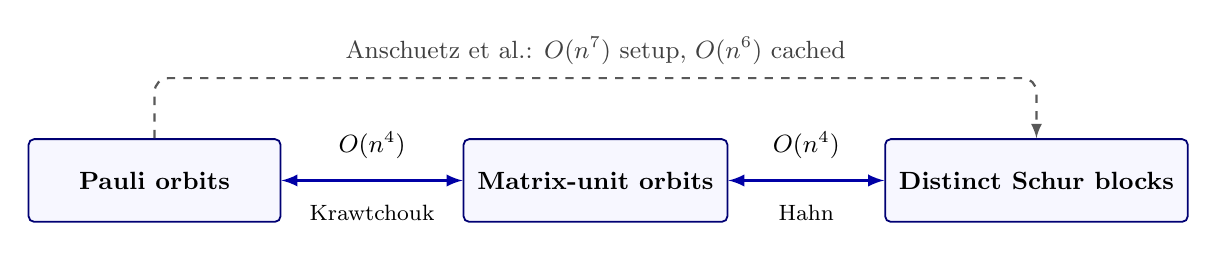
\begin{tikzpicture}[
    font=\small,
    coordinate box/.style={
        draw=blue!45!black, fill=blue!3, rounded corners=2pt,
        line width=0.65pt, minimum width=3.2cm, minimum height=1.05cm,
        align=center, inner sep=5pt
    },
    thesis arrow/.style={<->, >=latex, draw=blue!65!black, line width=1pt}
]
    \node[coordinate box] (pauli) at (0,0)
        {\textbf{Pauli orbits}};
    \node[coordinate box] (matrix) at (5.6,0)
        {\textbf{Matrix-unit orbits}};
    \node[coordinate box] (schur) at (11.2,0)
        {\textbf{Distinct Schur blocks}};

    \draw[->, >=latex, dashed, draw=black!65, line width=0.8pt,
          rounded corners=5pt]
        (pauli.north) -- (0,1.3) -- (11.2,1.3) -- (schur.north);
    \node[above, text=black!75] at (5.6,1.35)
        {Anschuetz et al.: $O(n^7)$ setup, $O(n^6)$ cached};

    \draw[thesis arrow] (pauli.east) --
        node[above=4pt] {$O(n^4)$}
        node[below=5pt, font=\footnotesize] {Krawtchouk} (matrix.west);
    \draw[thesis arrow] (matrix.east) --
        node[above=4pt] {$O(n^4)$}
        node[below=5pt, font=\footnotesize] {Hahn} (schur.west);

\end{tikzpicture}
